\documentclass[a4paper, 12pt]{article}%тип документа

%отступы
\usepackage[left=2cm,right=2cm,top=2cm,bottom=3cm,bindingoffset=0cm]{geometry}

%Русский язык
\usepackage[T2A]{fontenc} %кодировка
\usepackage[utf8]{inputenc} %кодировка исходного кода
\usepackage[english,russian]{babel} %локализация и переносы

%Вставка картинок
\usepackage{wrapfig}
\usepackage{graphicx}
\graphicspath{{pictures/}}
\DeclareGraphicsExtensions{.pdf,.png,.jpg}
\usepackage{subfig}

%Графики
\usepackage{multirow}
\usepackage{pgfplots}
\usepackage{rotating}
\usepackage{pgfplotstable}
\usepackage{booktabs}
\usepackage{multirow}
\pgfplotsset{compat=1.9}

%Математика
\usepackage{amsmath, amsfonts, amssymb, amsthm, mathtools}

%Заголовок
\author{Сифат Мд Абдуллах Ал Хасиб \\
Физтех школа электроники, фотоники и молекулярной физики \\
Группа Б04-105}
\title{\textbf{Лаборатория Работа 2.1.3 \\ 
Определение $C_p/C_v$ по скорости звука в газе}}
\begin{document}
\maketitle
\section{Введение}\textbf{Цель работы:} 1) измерение частоты колебаний и длины волны при резонансе звуковых колебаний в газе, заполняющем трубу;
2) определение показателя адиабаты с помощью уравнения состояния идеального газа\\
\textbf{В работе используется:} звуковой генератор, электронный осциллограф, теплоизолированная труба, обогреваемая водой из термостата, термостат, телефон, соединённый с генератором звука, микрофон, соединённый с осциллографом.
\section{Теоретическая справка}
Скорость распространения звуковой волны в газах зависит от показателя адиабаты $\gamma$. На измерении скорости звука основан один из наиболее точных методов определения показателя адиабаты.

Скорость звука в газах определяется формулой:
\[
	c = \sqrt{\gamma \frac{RT}{\mu}},
\]
где $R$ --- газовая постоянная, $T$ --- температура газа, а $\mu$ --- его молярная масса. Преобразуя эту формулу, найдем
\begin{equation}
	\gamma = \frac{\mu}{RT} c^2.
\end{equation}
Таким образом, для определения показателя адиабаты достаточно измерить температуру газа и скорость распространения звука (молярная масса газа предполагается известной).

Звуковая волна, распространяющаяся вдоль трубы, испытывает
многократные отражения от торцов. Звуковые колебания в трубе являются наложением всех отраженных волн и, вообще говоря, очень сложны. Картина упрощается, если длина трубы $L$ равна целому числу полуволн, то есть когда
\begin{equation}
	L = n \lambda/2,
\end{equation}
где $\lambda$ --- длина волны звука в трубе, а $n$ --- любое целое число. Если условие (2) выполнено, то волна, отраженная от торца трубы, вернувшаяся к ее началу и вновь отраженная, совпадает по фазе с падающей. Совпадающие по фазе волны усиливают друг друга. Амплитуда звуковых колебаний при этом резко возрастает --- наступает
резонанс.
При звуковых колебаниях слои газа, прилегающие к торцам трубы, не испытывают смещения (\itshape узел смещения\rm ). Узлы смещения повторяются по всей длине трубы через $\lambda/2$. Между узлами находятся
максимумы смещения (\itshape пучности\rm ).

Скорость звука c связана с его частотой $f$ и длиной волны $\lambda$ соотношением
\begin{equation}
	c = \lambda f.
\end{equation}
Для получения резонанса при постоянной длине трубы можно изменять частоту звуковых колебаний. В этом случае следует плавно изменять частоту $f$
звукового генератора, а следовательно, и длину звуковой волны $\lambda$.
Для последовательных резонансов получим
\begin{equation}
L_n = \frac{\lambda_1}{2}n=\frac{\lambda_2}{2}(n+1) = \ldots = \frac{\lambda_{k+1}}{2}(n+k)
\end{equation}
Из (3) и (4) имеем
\[
	f_1 = \frac{c}{\lambda_1} = \frac{c}{2L}n, \quad f_2 = \frac{c}{\lambda_2} = \frac{c}{2L}(n+1) = f_1 + \frac{c}{2L},\quad \ldots,
\]
\begin{equation}
f_{k+1} = \frac{c}{\lambda_{k+1}} = \frac{c}{2L}(n+k)= f_1 + \frac{c}{2L}k.
\end{equation}\\
Скорость звука, деленная на $2L$, определяется, таким образом,
по угловому коэффициенту графика зависимости частоты от номера
резонанса.

\section{Экспериментальная установка:}
В нашей работе мы использовали следующую экспериментальную установку. Где звуковые колебания в трубе возбуждаются телефоном Т и улавливаются микрофоном М. Мембрана телефона приводится в движение переменным током звуковой частоты; в качестве источника переменной ЭДС используется звуковой генератор ГЗ. Возникающий в микрофоне сигнал наблюдается на осциллографе ЭТО. Микрофон и телефон присоединены к установке через тонкие резиновые трубки. Такая связь достаточна для возбуждения и обнаружения звуковых колебаний в трубе и в то же время мало возмущает эти колебания: при расчётах оба торца трубы можно считать неподвижными, авлиянием соединительных отверстий пренебречь.\\
\linebreak Эта установка (рис. 1) содержит теплоизолированную трубу постоянной длины. Воздух в трубе нагревается водой из термостата. Температура газа принимается равной температуре воды, омывающей трубу. На этой установке измеряется зависимость скорости звука от температуры.

\begin{figure}[h]
\begin{center}
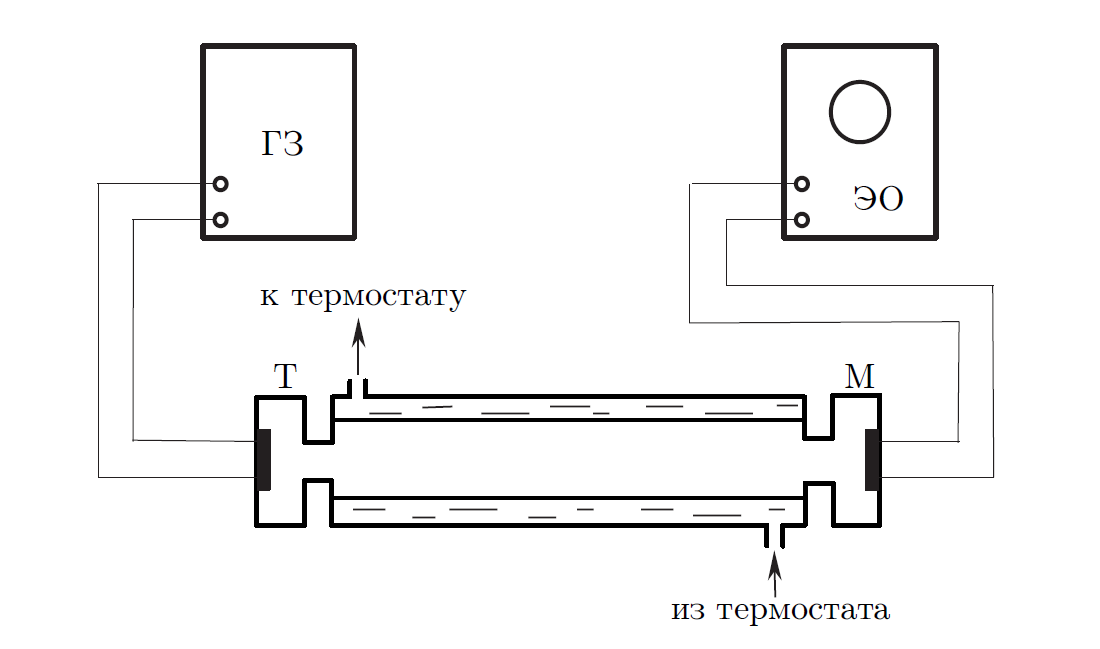
\includegraphics[width = 0.9\textwidth]{fig1.png}
\caption{Схема установки}
\end{center}
\end{figure}

\newpage
\section{Ход работы}
Мы провели эксперимент с воздухом внутри трубы длиной $740 \pm 1$
 мм. Температура в помещении в день эксперимента составляла 23°C. Скорость звука при этой температуре составляла 340 м/с. Hаш эксперимент был при 6 различных температурах и записали резонансную частоту звука в воздухе внутри трубы.\\

\begin{center}
\begin{tabular}{|c|c|c|c|c|c|}
\hline
$T_1, K$ & $T_2, K$ & $T_3, K$ & $T_4, K$ & $T_5, K$ & $T_6, K$ \\\hline
$296$ & $301$ & $306.1$ & $311.2$ & $316.1$ & $321$ \\\hline
\end{tabular}
\end{center}
\begin{center}
\begin{tabular}{|c|c|c|c|c|c|c|}
\hline
$T_1$ & $f_1,\ \text{Гц}$ &$f_2,\ \text{Гц}$ &$f_3,\ \text{Гц}$ &$f_4,\ \text{Гц}$ &$f_5,\ \text{Гц}$ & $f_6,\ \text{Гц}$\\\hline
 $$ & $251$ & $477$ & $708$ & $928$ & $1163$ & $1393$ \\\hline
\end{tabular}
\end{center}
\begin{center}
\begin{tabular}{|c|c|c|c|c|c|c|}
\hline
$T_2$ & $f_1,\ \text{Гц}$ &$f_2,\ \text{Гц}$ &$f_3,\ \text{Гц}$ &$f_4,\ \text{Гц}$ &$f_5,\ \text{Гц}$ & $f_6,\ \text{Гц}$\\\hline
 $$ & $257$ & $484$ & $716$ & $945$ & $1170$ & $1404$ \\\hline
\end{tabular}
\end{center}
\begin{center}
\begin{tabular}{|c|c|c|c|c|c|c|}
\hline
$T_3$ & $f_1,\ \text{Гц}$ &$f_2,\ \text{Гц}$ &$f_3,\ \text{Гц}$ &$f_4,\ \text{Гц}$ &$f_5,\ \text{Гц}$ & $f_6,\ \text{Гц}$\\\hline
 $$ & $252$ & $486$ & $720$ & $948$ & $1182$ & $1418$ \\\hline
\end{tabular}
\end{center}
\begin{center}
\begin{tabular}{|c|c|c|c|c|c|c|}
\hline
$T_4$ & $f_1,\ \text{Гц}$ &$f_2,\ \text{Гц}$ &$f_3,\ \text{Гц}$ &$f_4,\ \text{Гц}$ &$f_5,\ \text{Гц}$ & $f_6,\ \text{Гц}$\\\hline
 $$ & $252$ & $491$ & $724$ & $951$ & $1188$ & $1427$ \\\hline
\end{tabular}
\end{center}
\begin{center}
\begin{tabular}{|c|c|c|c|c|c|c|}
\hline
$T_5$ & $f_1,\ \text{Гц}$ &$f_2,\ \text{Гц}$ &$f_3,\ \text{Гц}$ &$f_4,\ \text{Гц}$ &$f_5,\ \text{Гц}$ & $f_6,\ \text{Гц}$\\\hline
 $$ & $255$ & $495$ & $731$ & $961$ & $1202$ & $1435$ \\\hline
\end{tabular}
\end{center}
\begin{center}
\begin{tabular}{|c|c|c|c|c|c|c|}
\hline
$T_6$ & $f_1,\ \text{Гц}$ &$f_2,\ \text{Гц}$ &$f_3,\ \text{Гц}$ &$f_4,\ \text{Гц}$ &$f_5,\ \text{Гц}$ & $f_6,\ \text{Гц}$\\\hline
 $$ & $260$ & $498$ & $734$ & $970$ & $1220$ & $1444$ \\\hline
\end{tabular}
\end{center}
\newpage Построим графики, откладывая по оси абсцисс номер резонанса $k$, а по оси ординат --- разность между частотой последующих резонансов и частотой первого резонанса:
$f_{k+1}-f_1$. Угловой коэффициент прямой определяет величину $c/2L$.

\begin{figure}[h]
\begin{center}
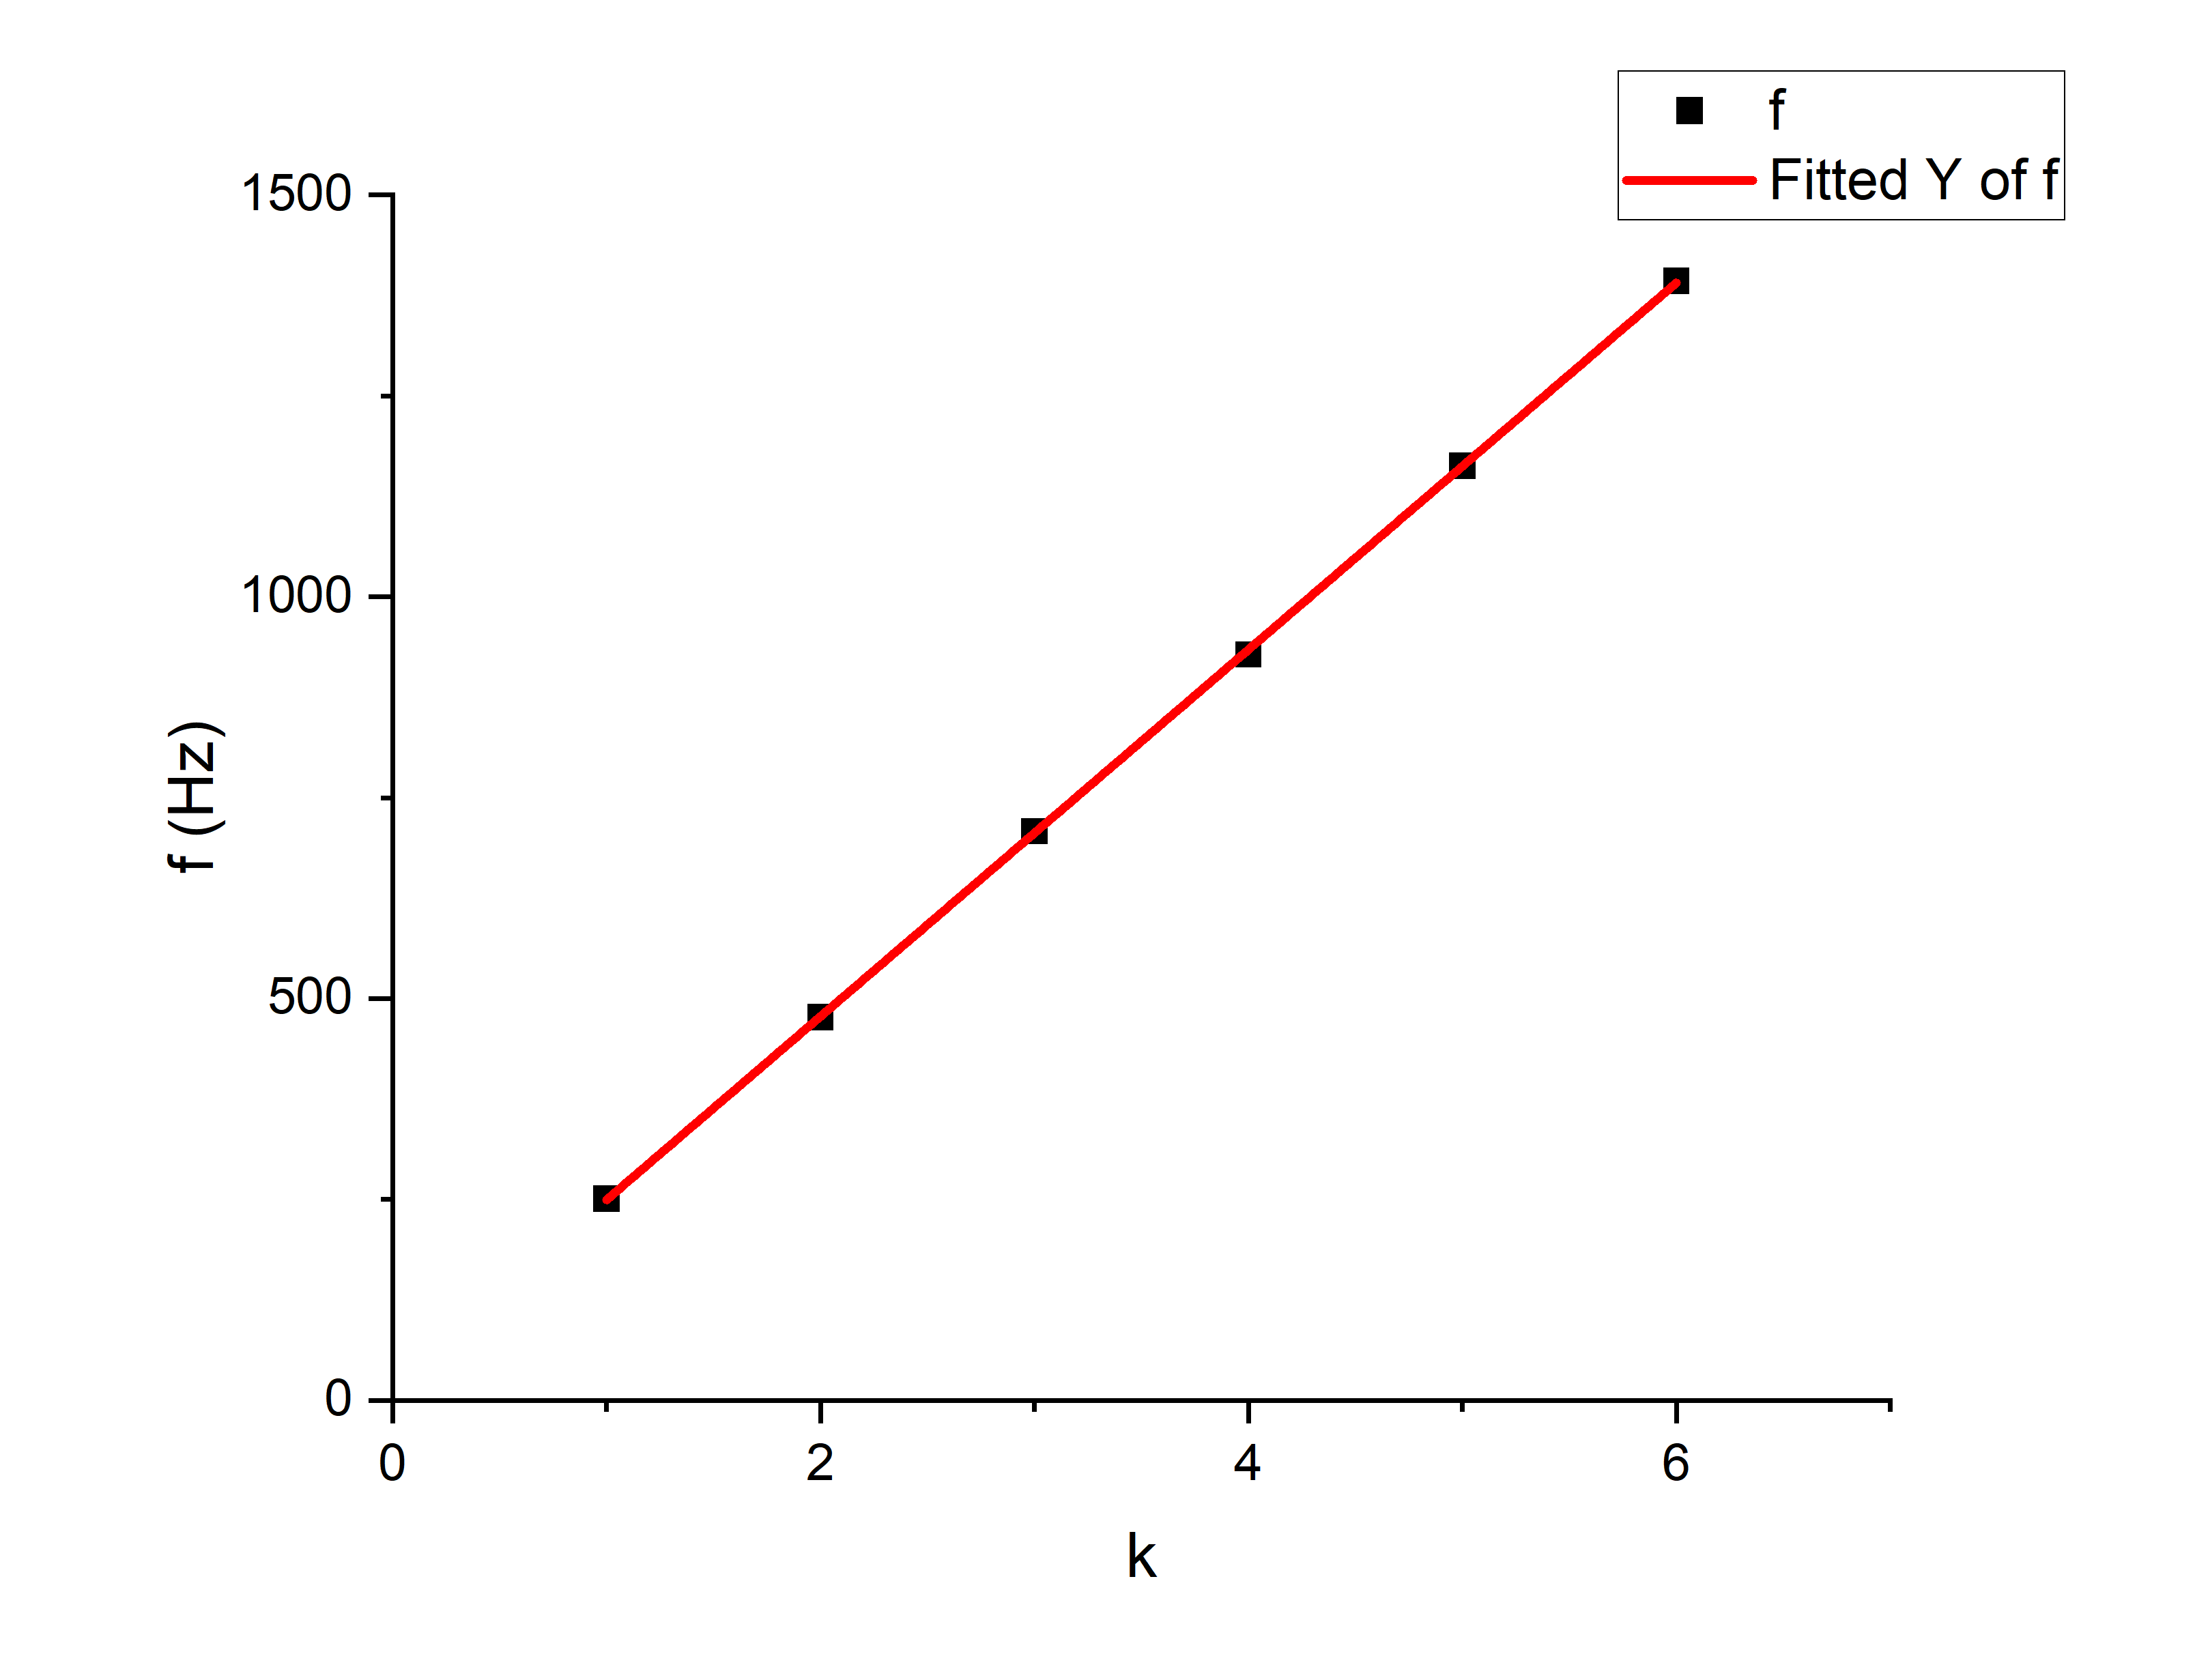
\includegraphics[width = 0.5\textwidth]{labphoto17.png}
\caption{График зависимости разности частот от номера резонанса при $T_1$}
\end{center}
\end{figure}

\begin{figure}[h]
\begin{center}
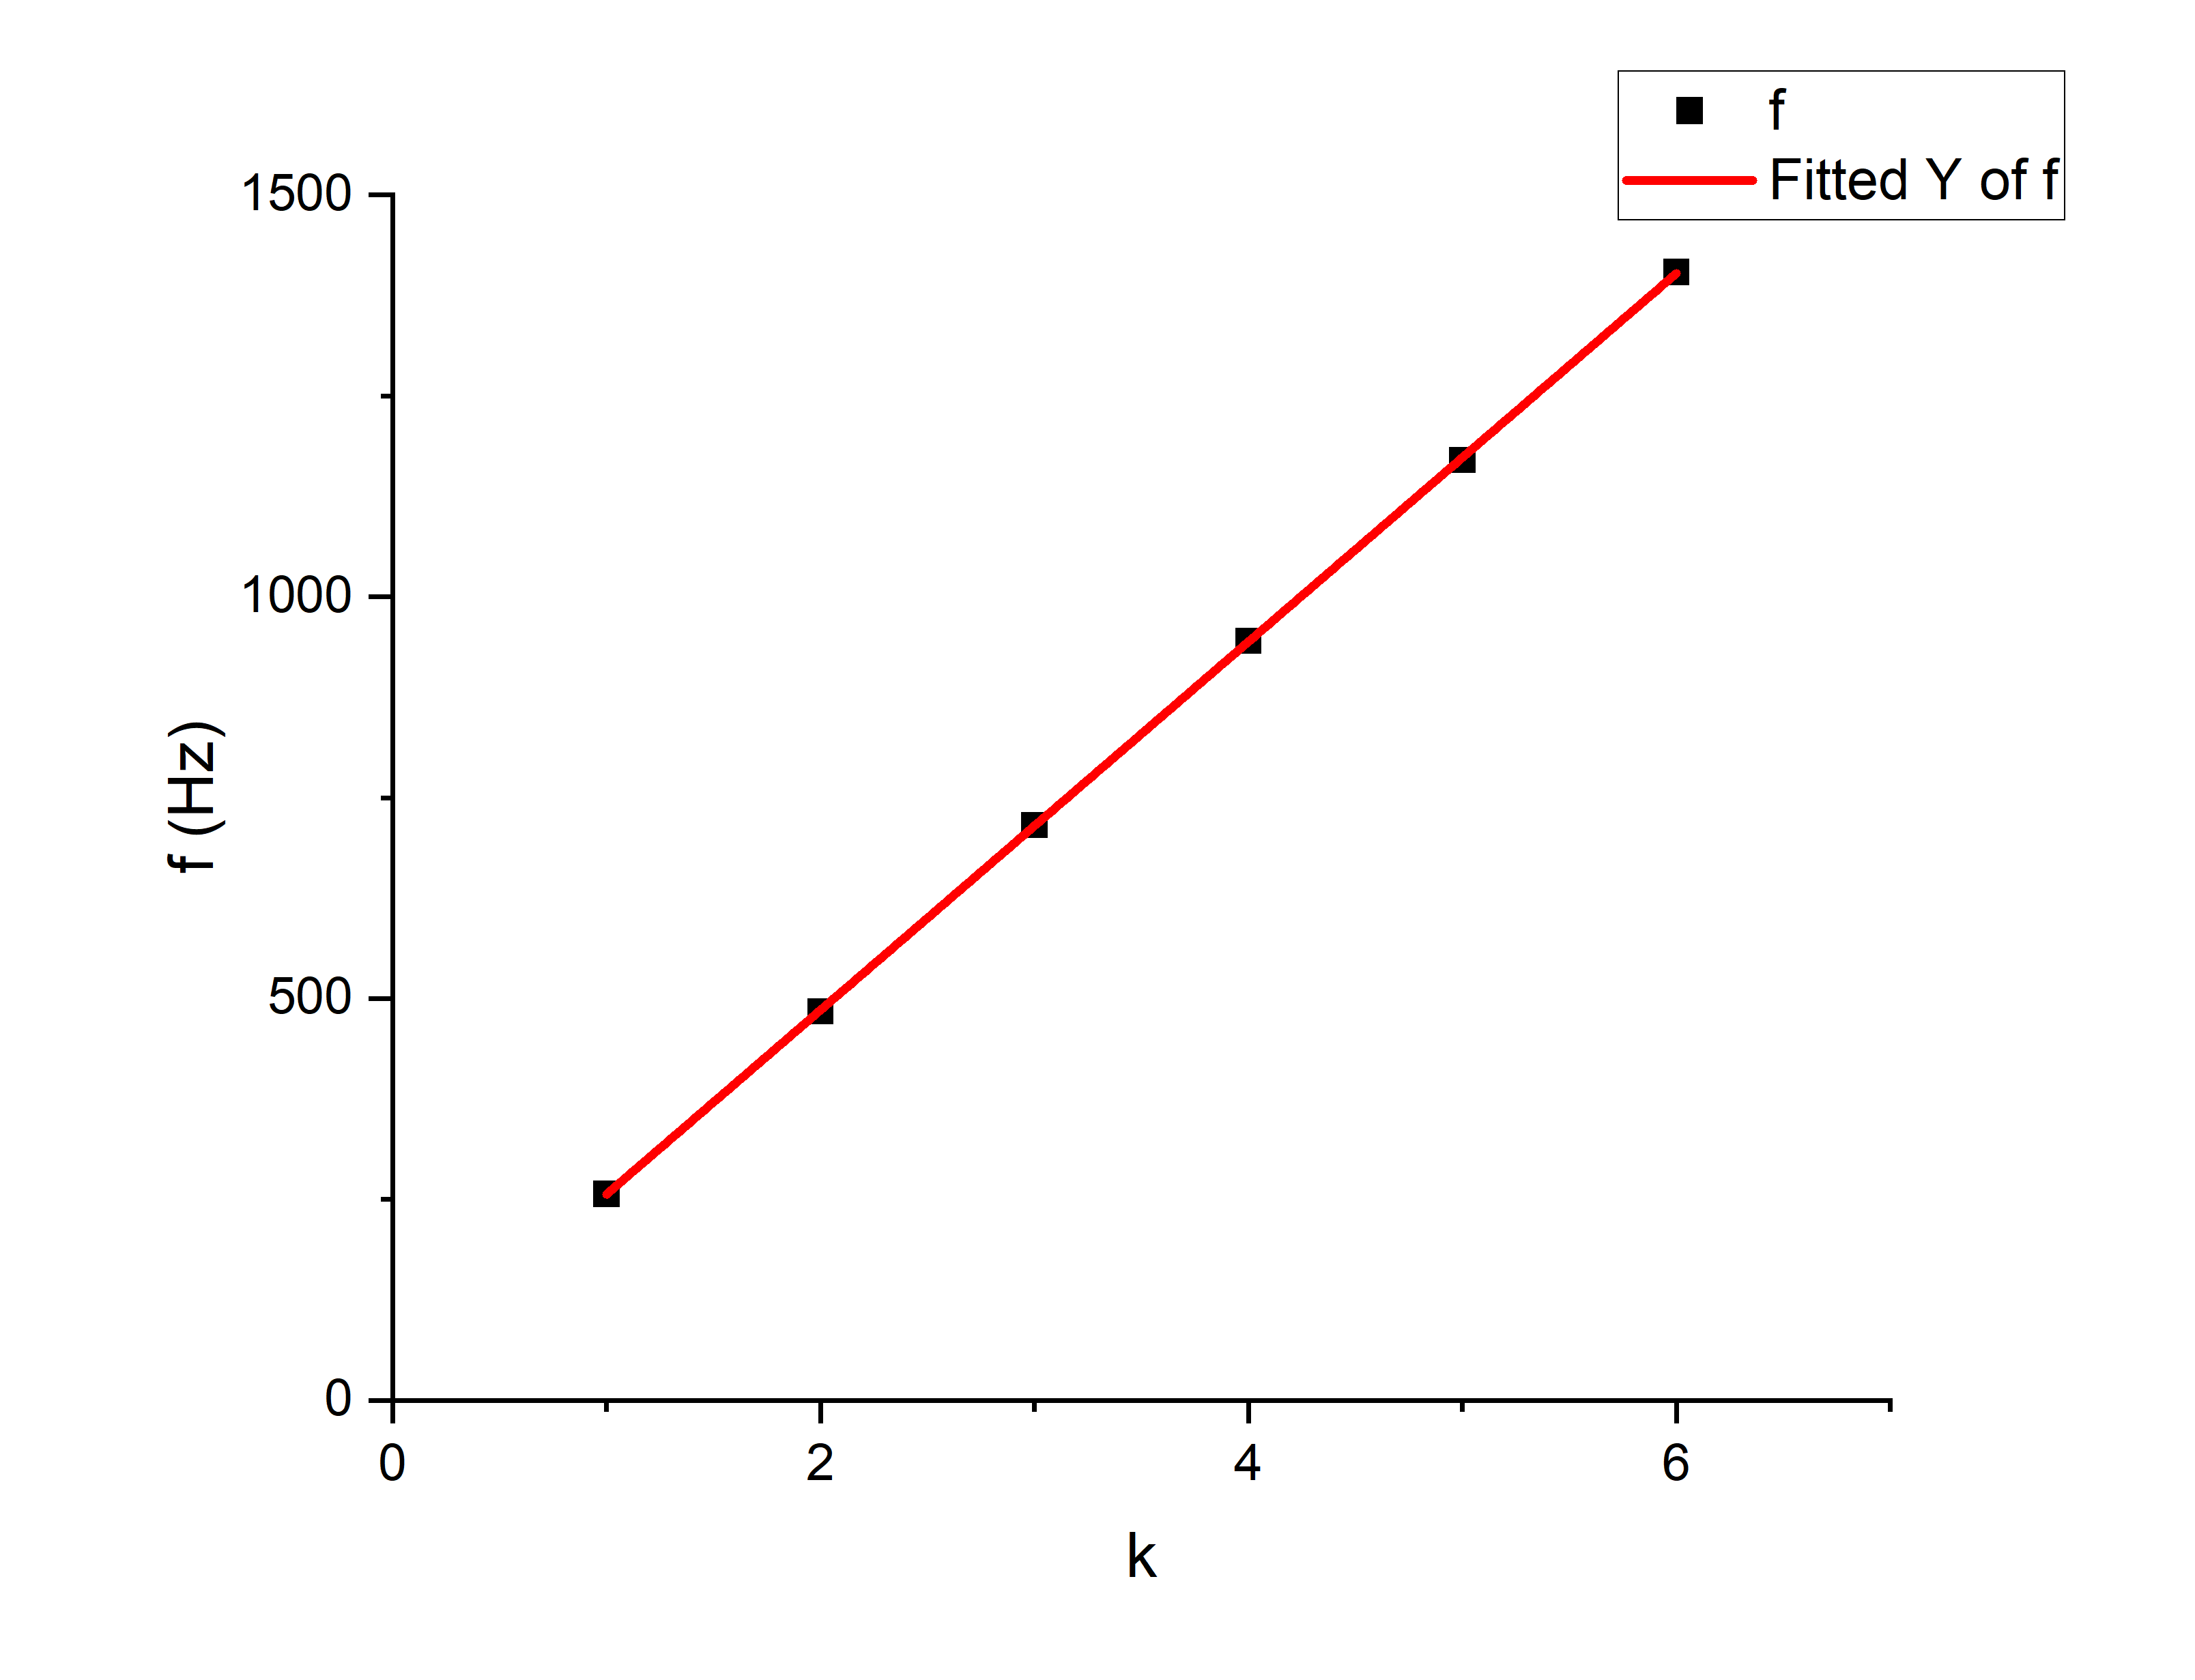
\includegraphics[width = 0.5\textwidth]{labphoto18.png}
\caption{График зависимости разности частот от номера резонанса при $T_2$}
\end{center}
\end{figure}

\begin{figure}
\begin{center}
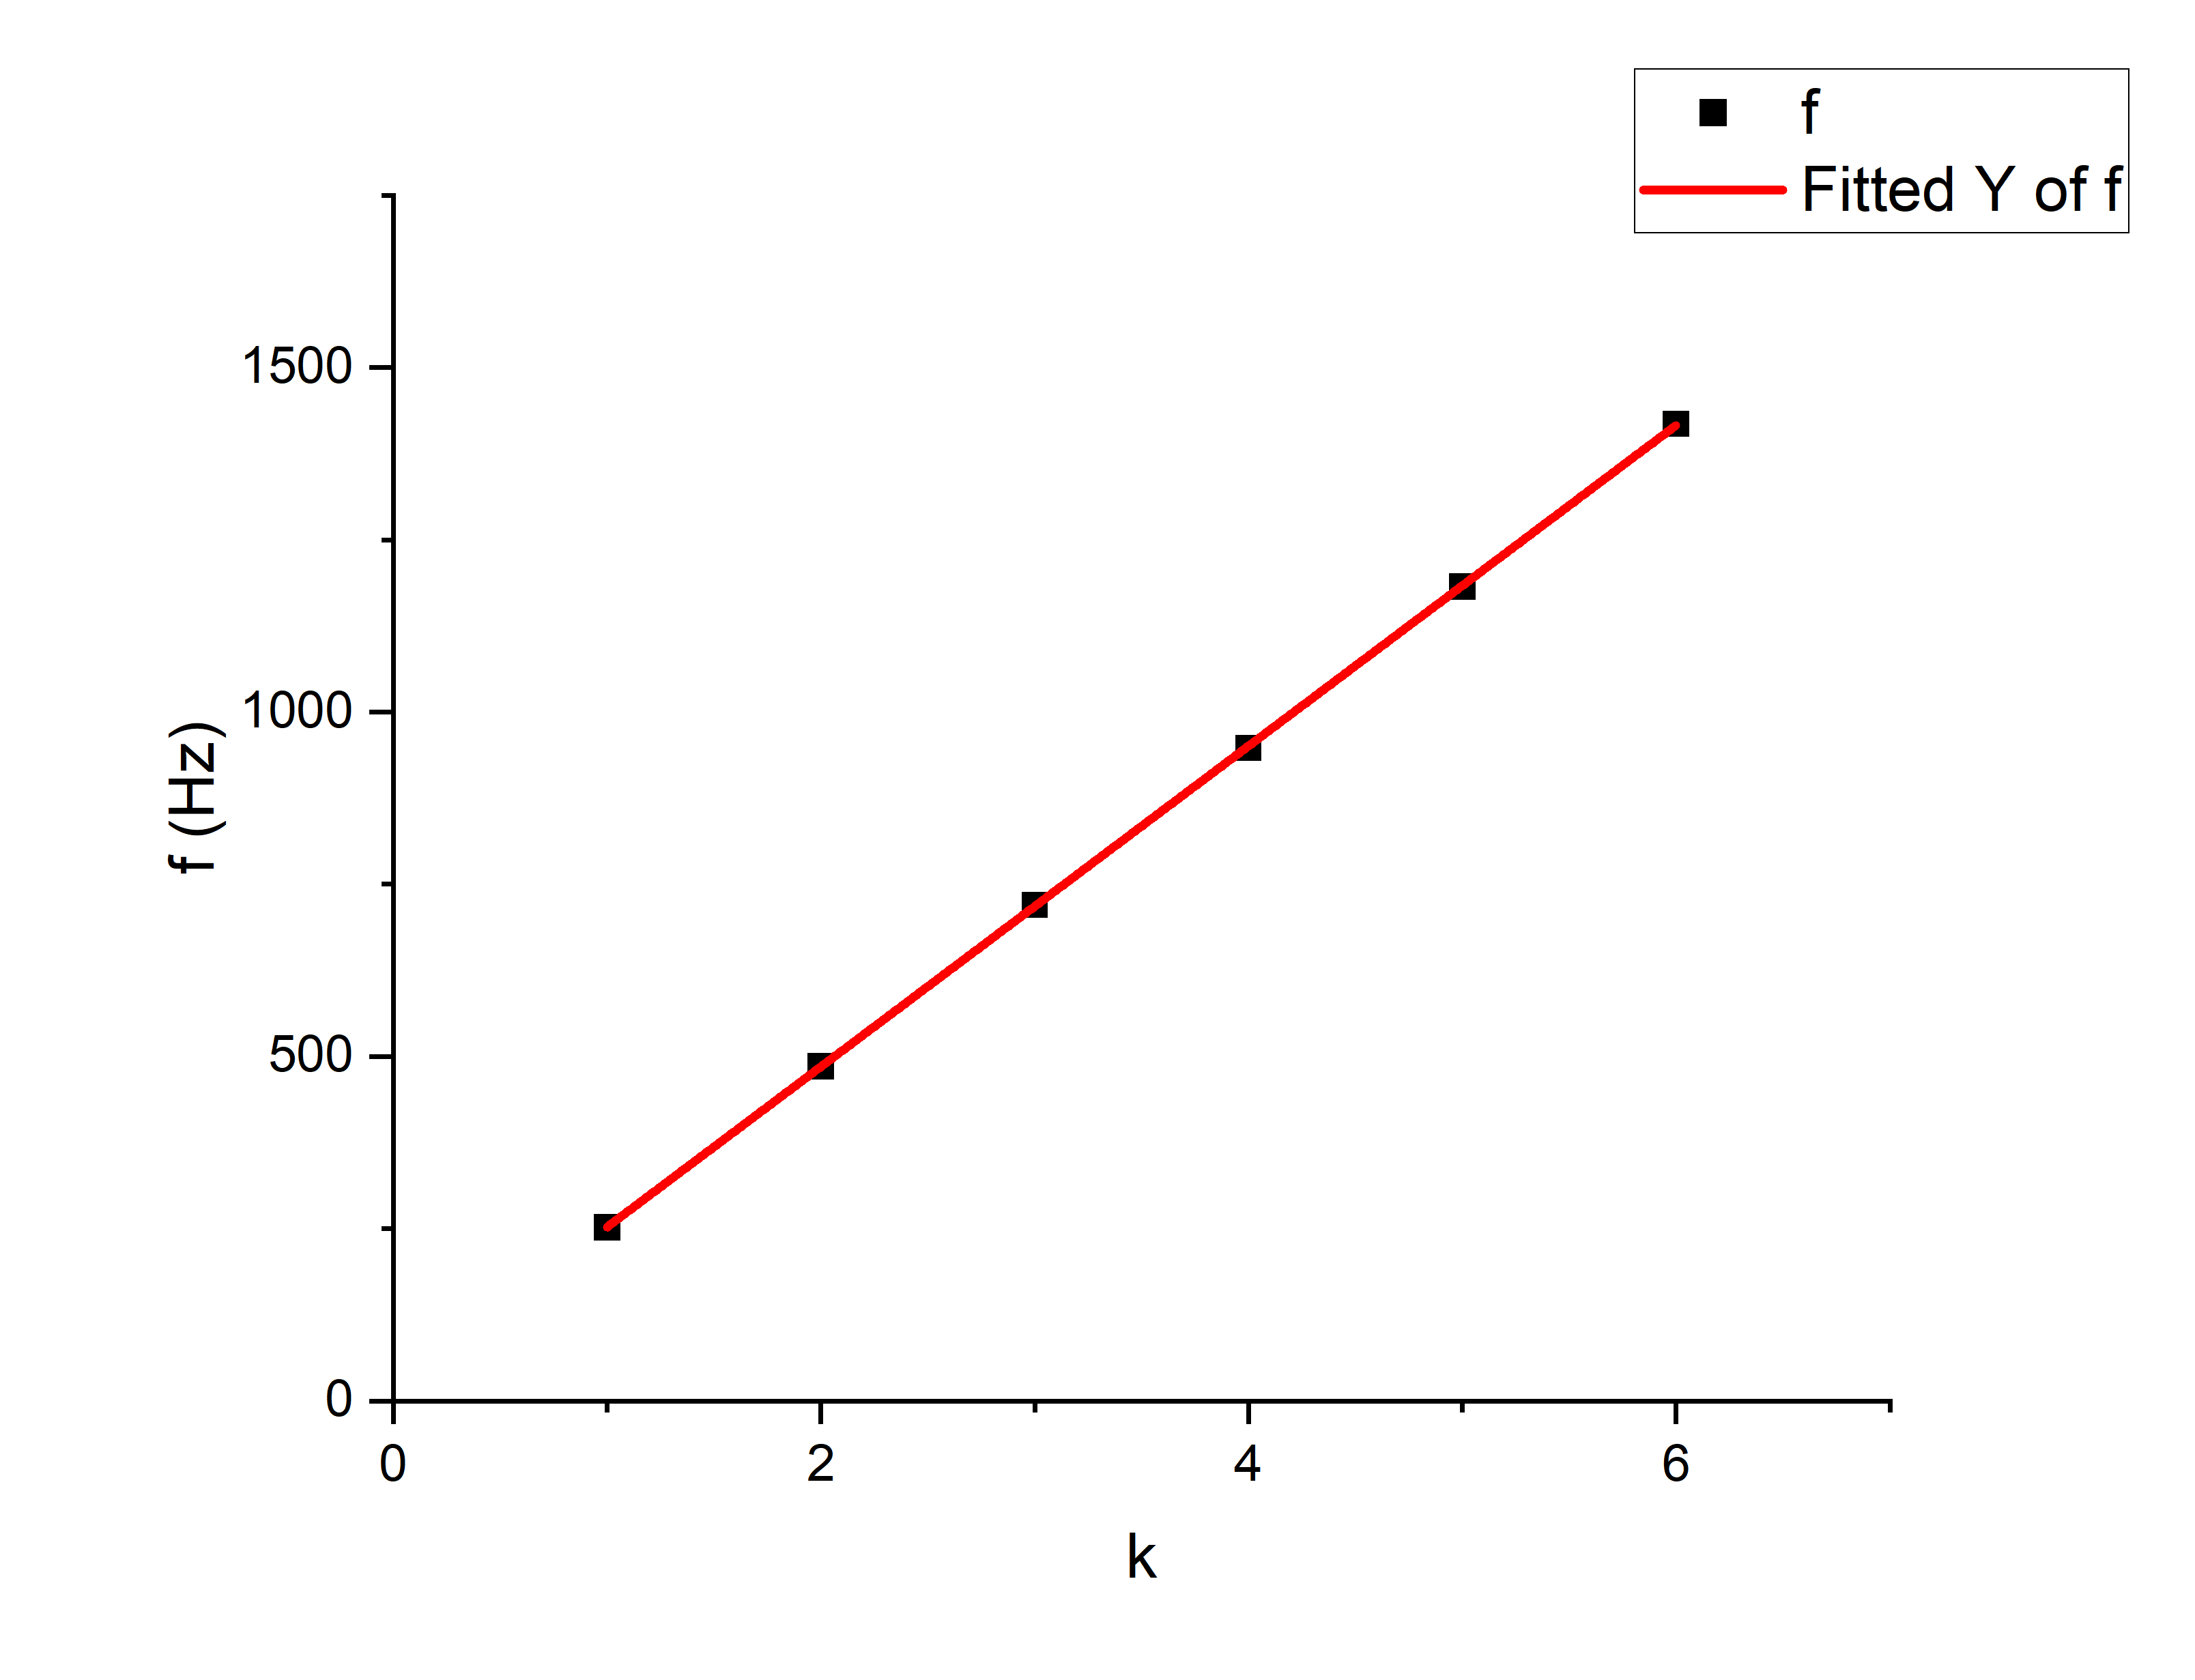
\includegraphics[width = 0.5\textwidth]{labphoto19.png}
\caption{График зависимости разности частот от номера резонанса при $T_3$}
\end{center}
\end{figure}

\begin{figure}
\begin{center}
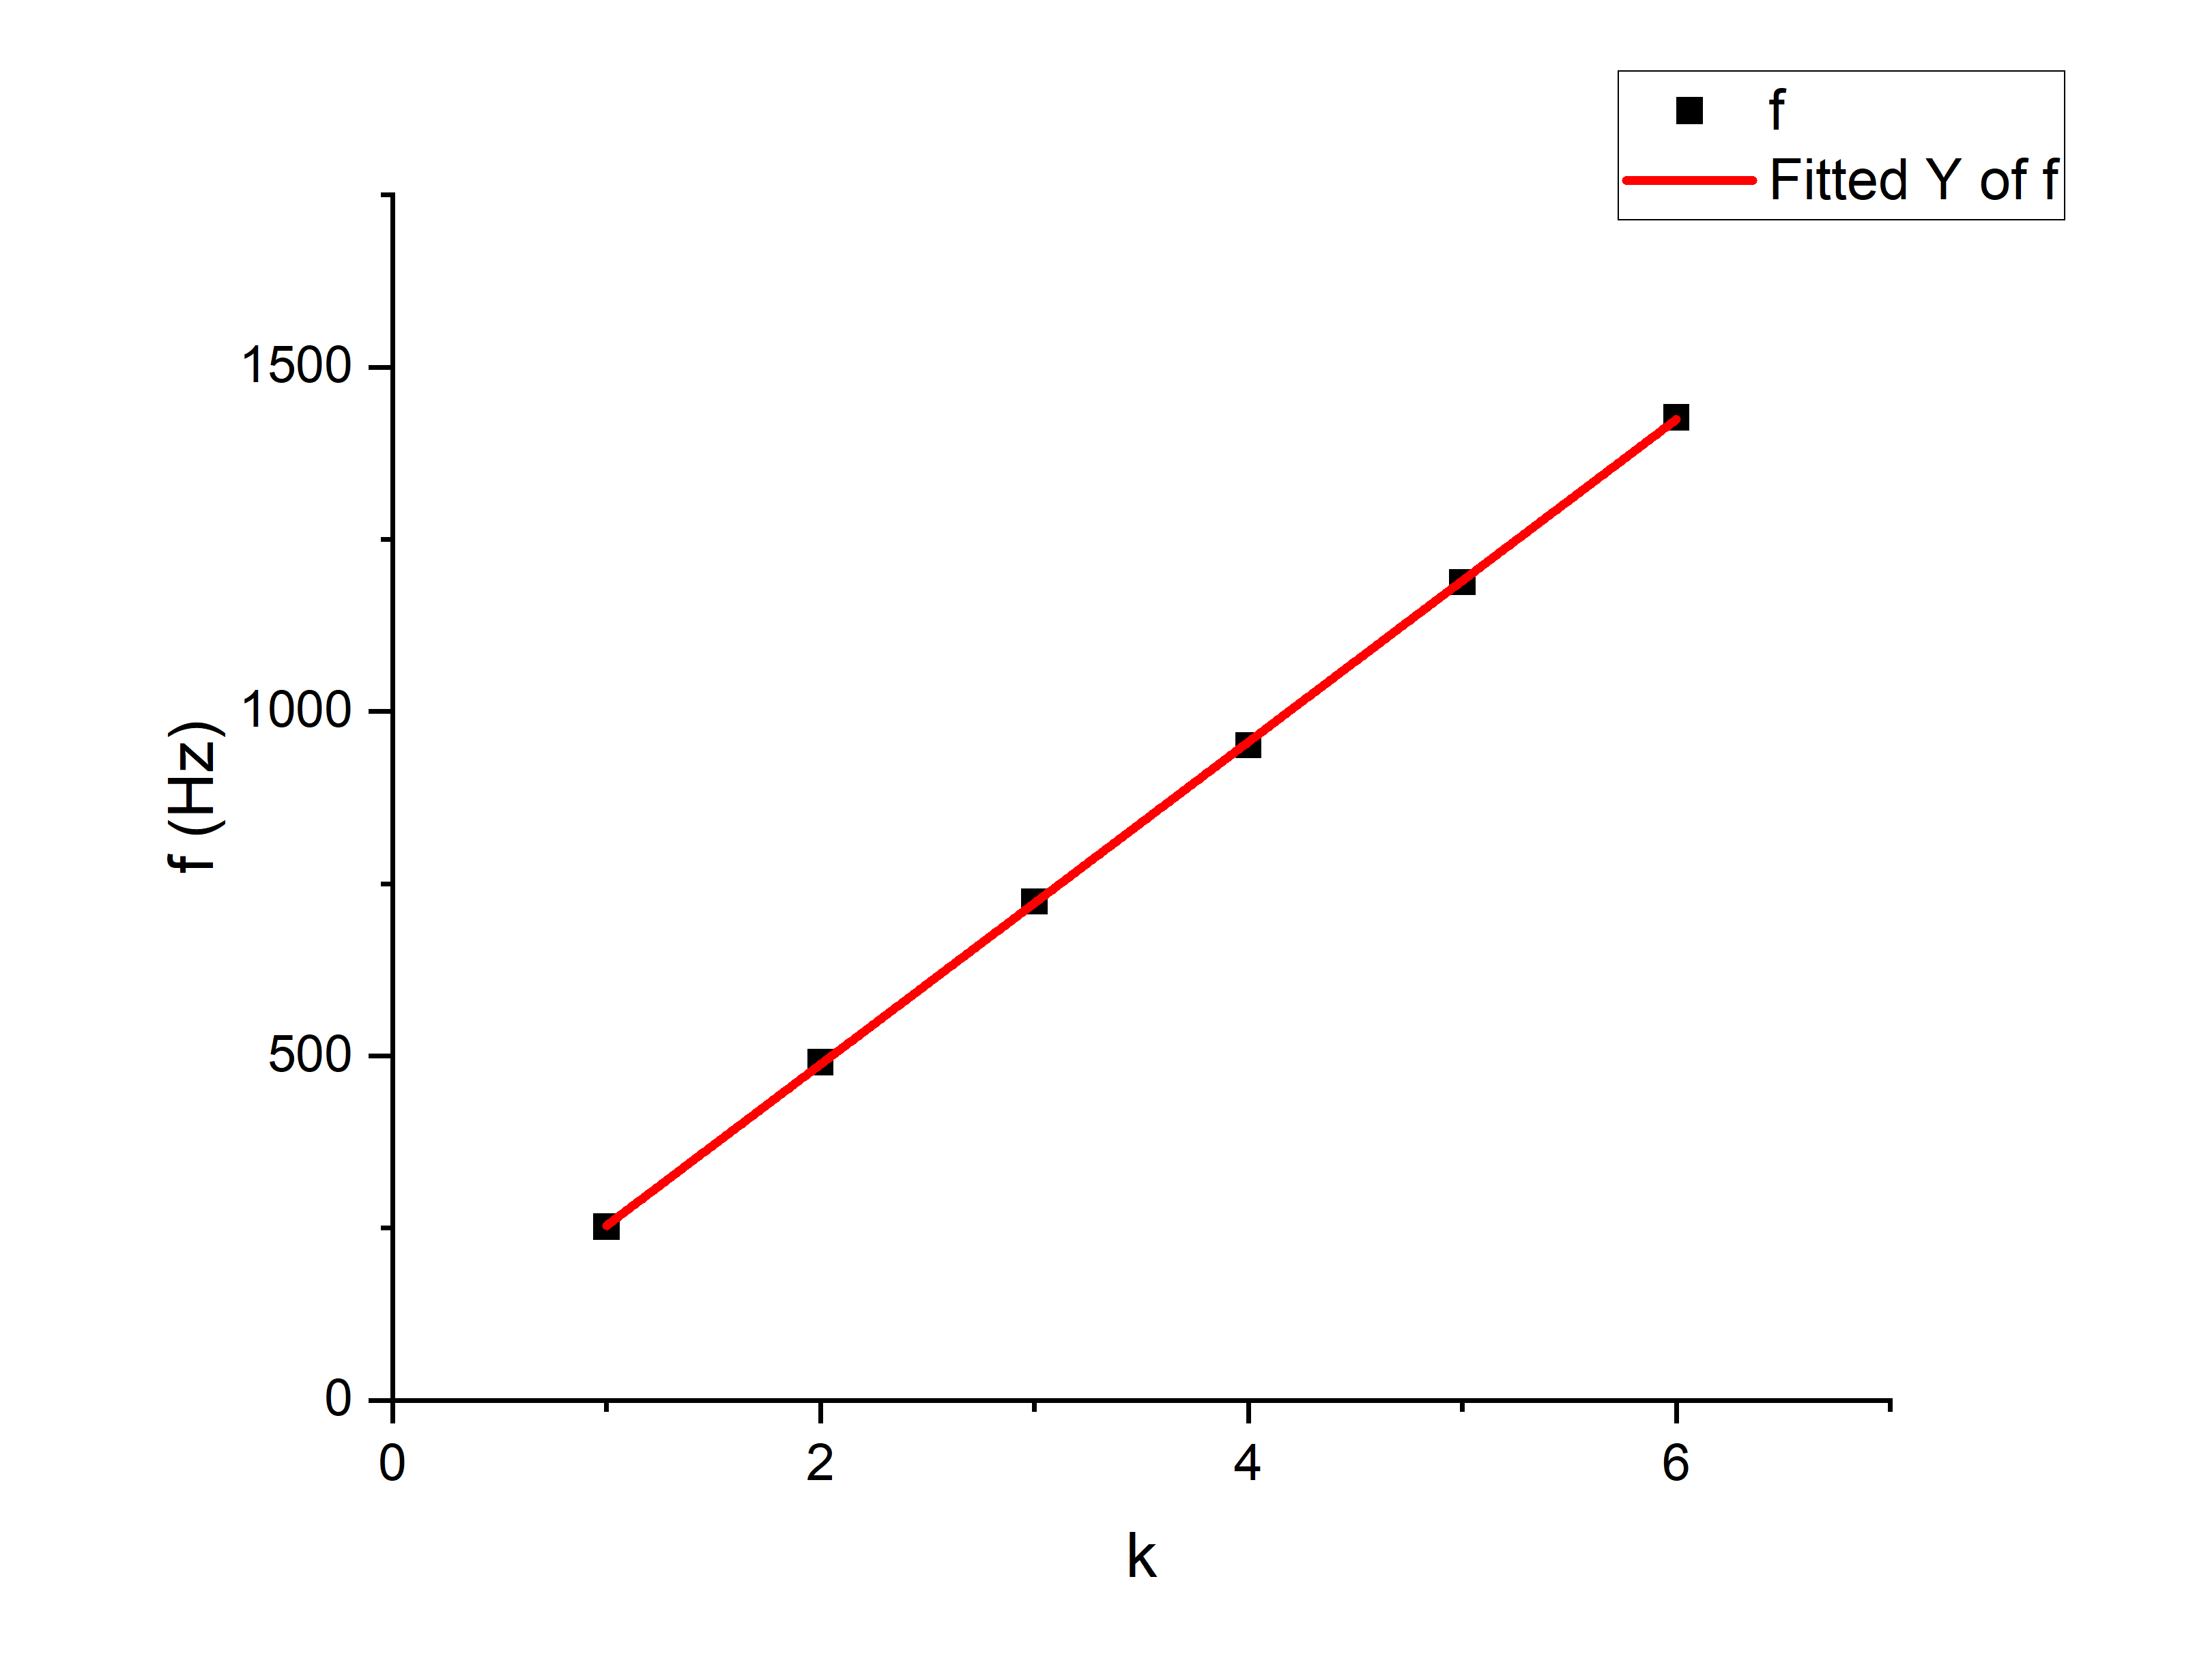
\includegraphics[width = 0.5\textwidth]{labphoto20.png}
\caption{График зависимости разности частот от номера резонанса при $T_4$}
\end{center}
\end{figure}

\begin{figure}
\begin{center}
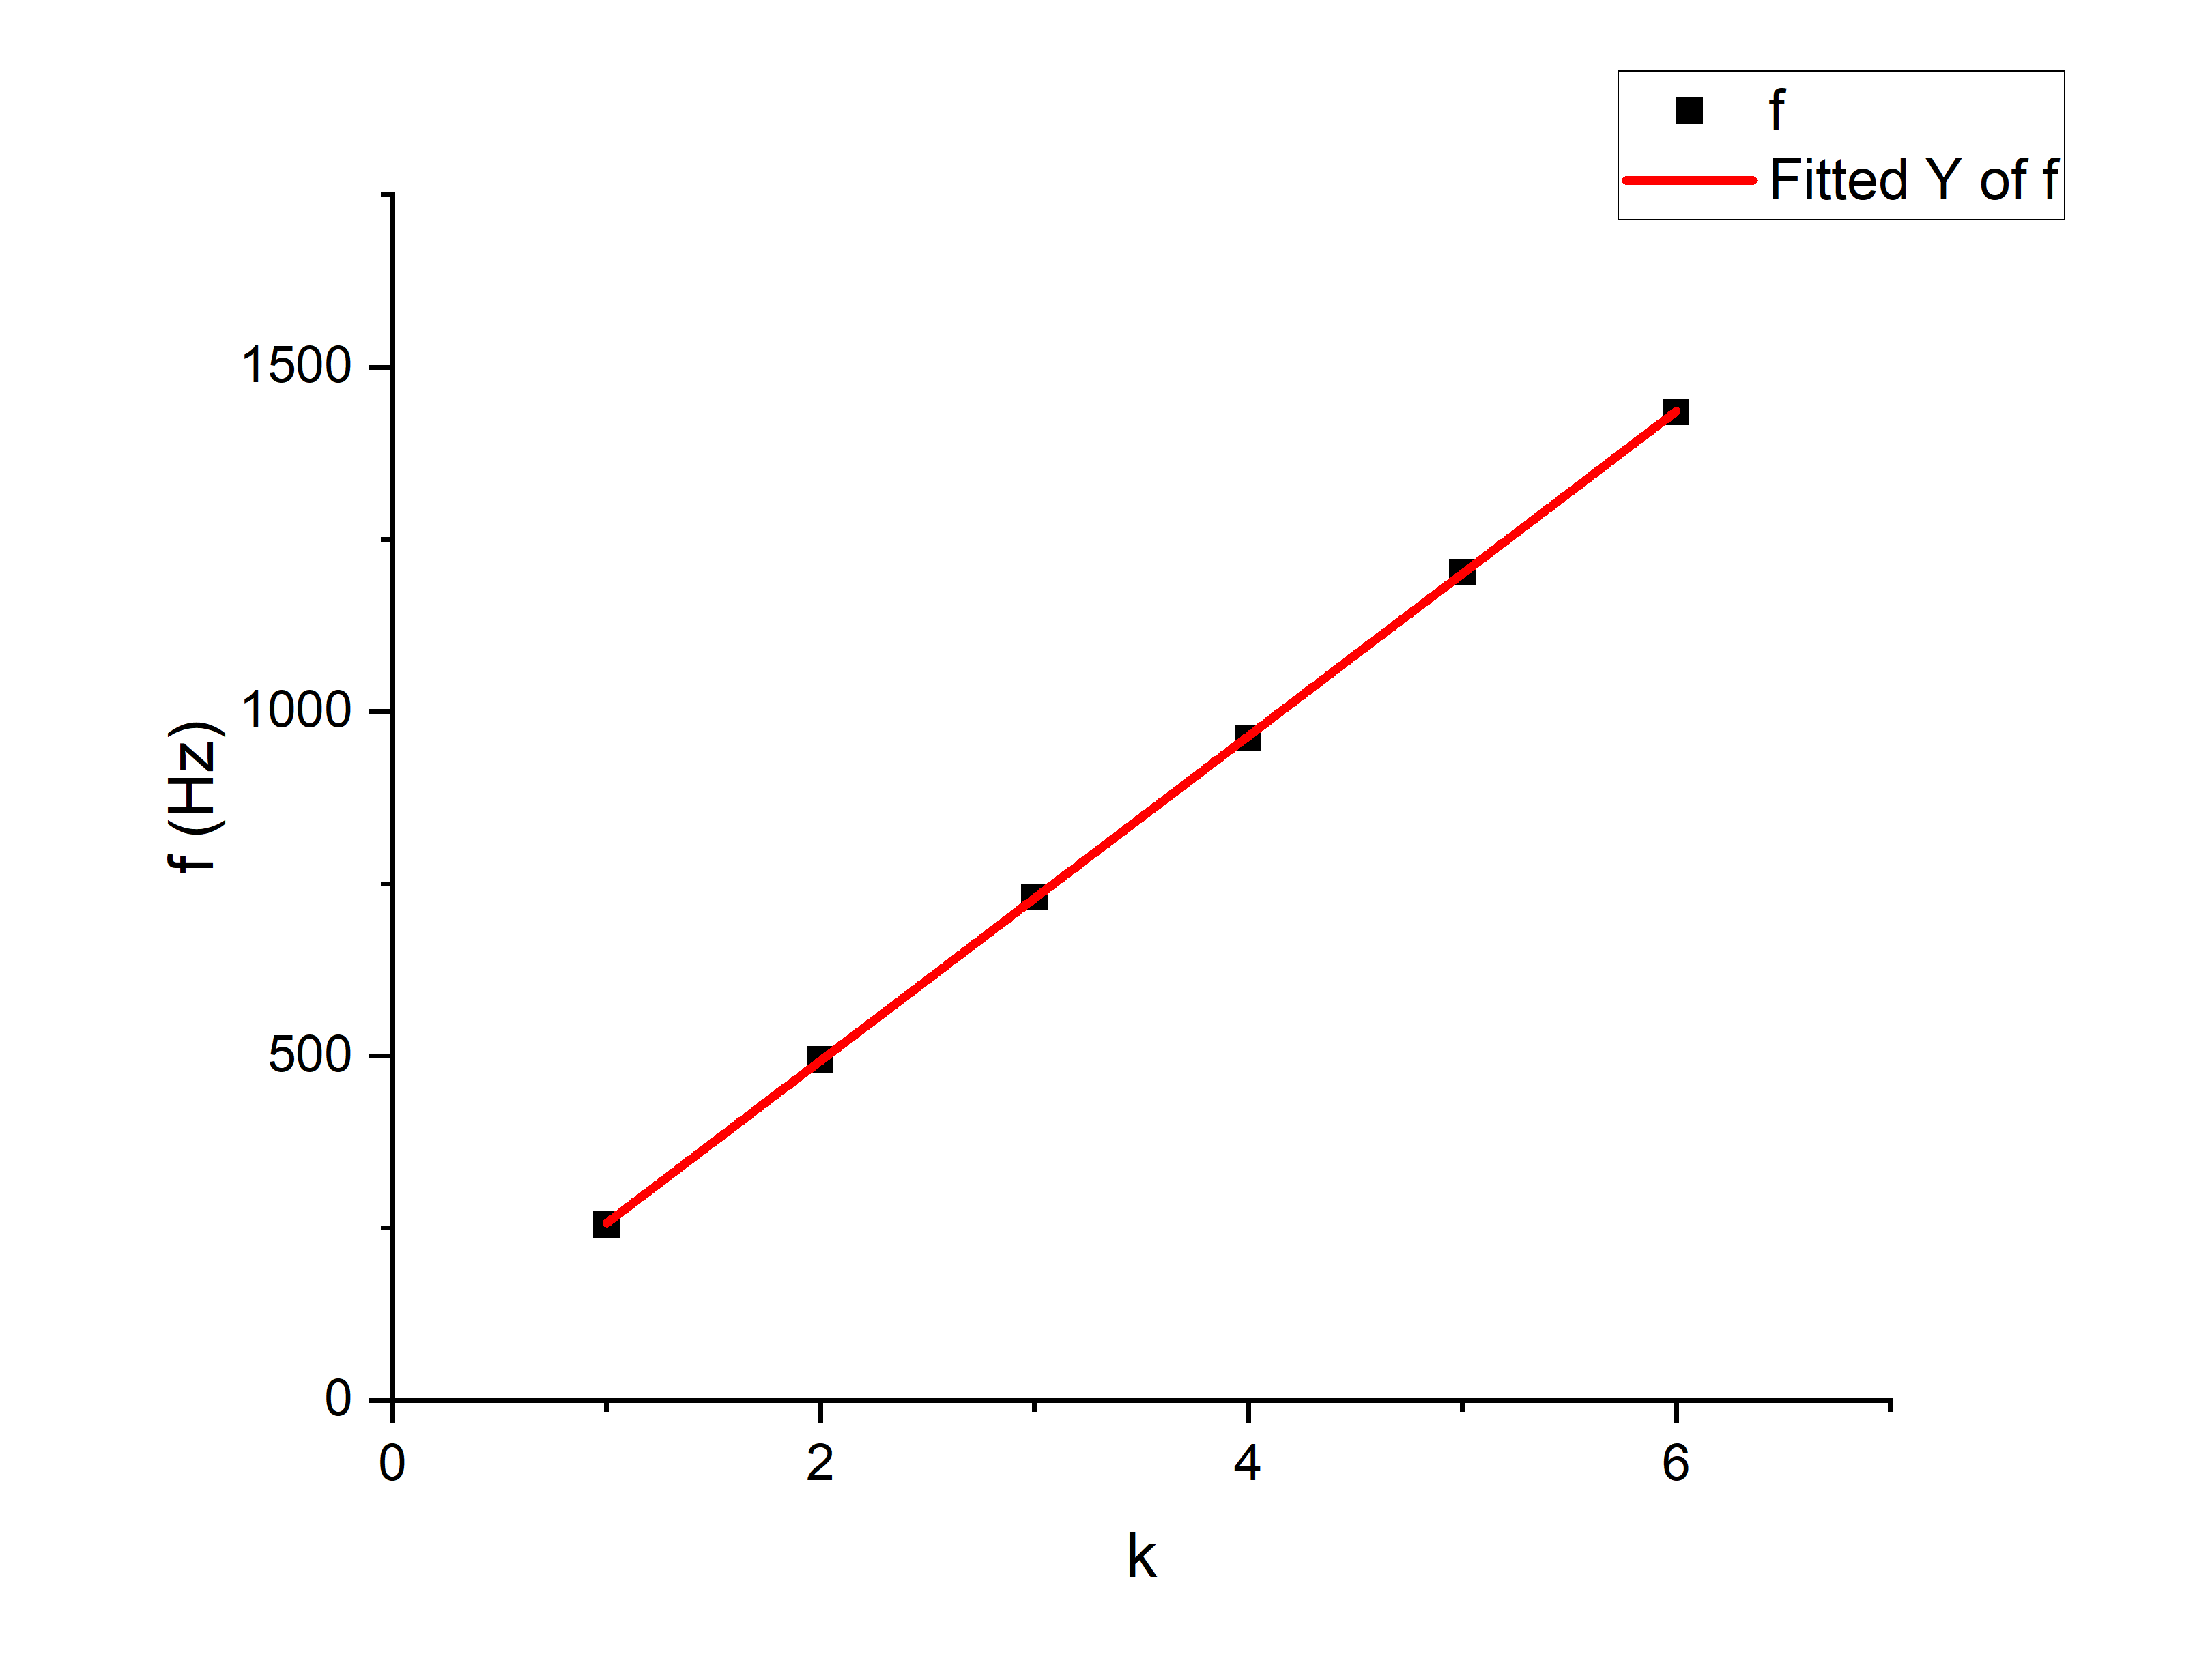
\includegraphics[width = 0.5\textwidth]{labphoto21.png}
\caption{График зависимости разности частот от номера резонанса при $T_5$}
\end{center}
\end{figure}

\begin{figure}
\begin{center}
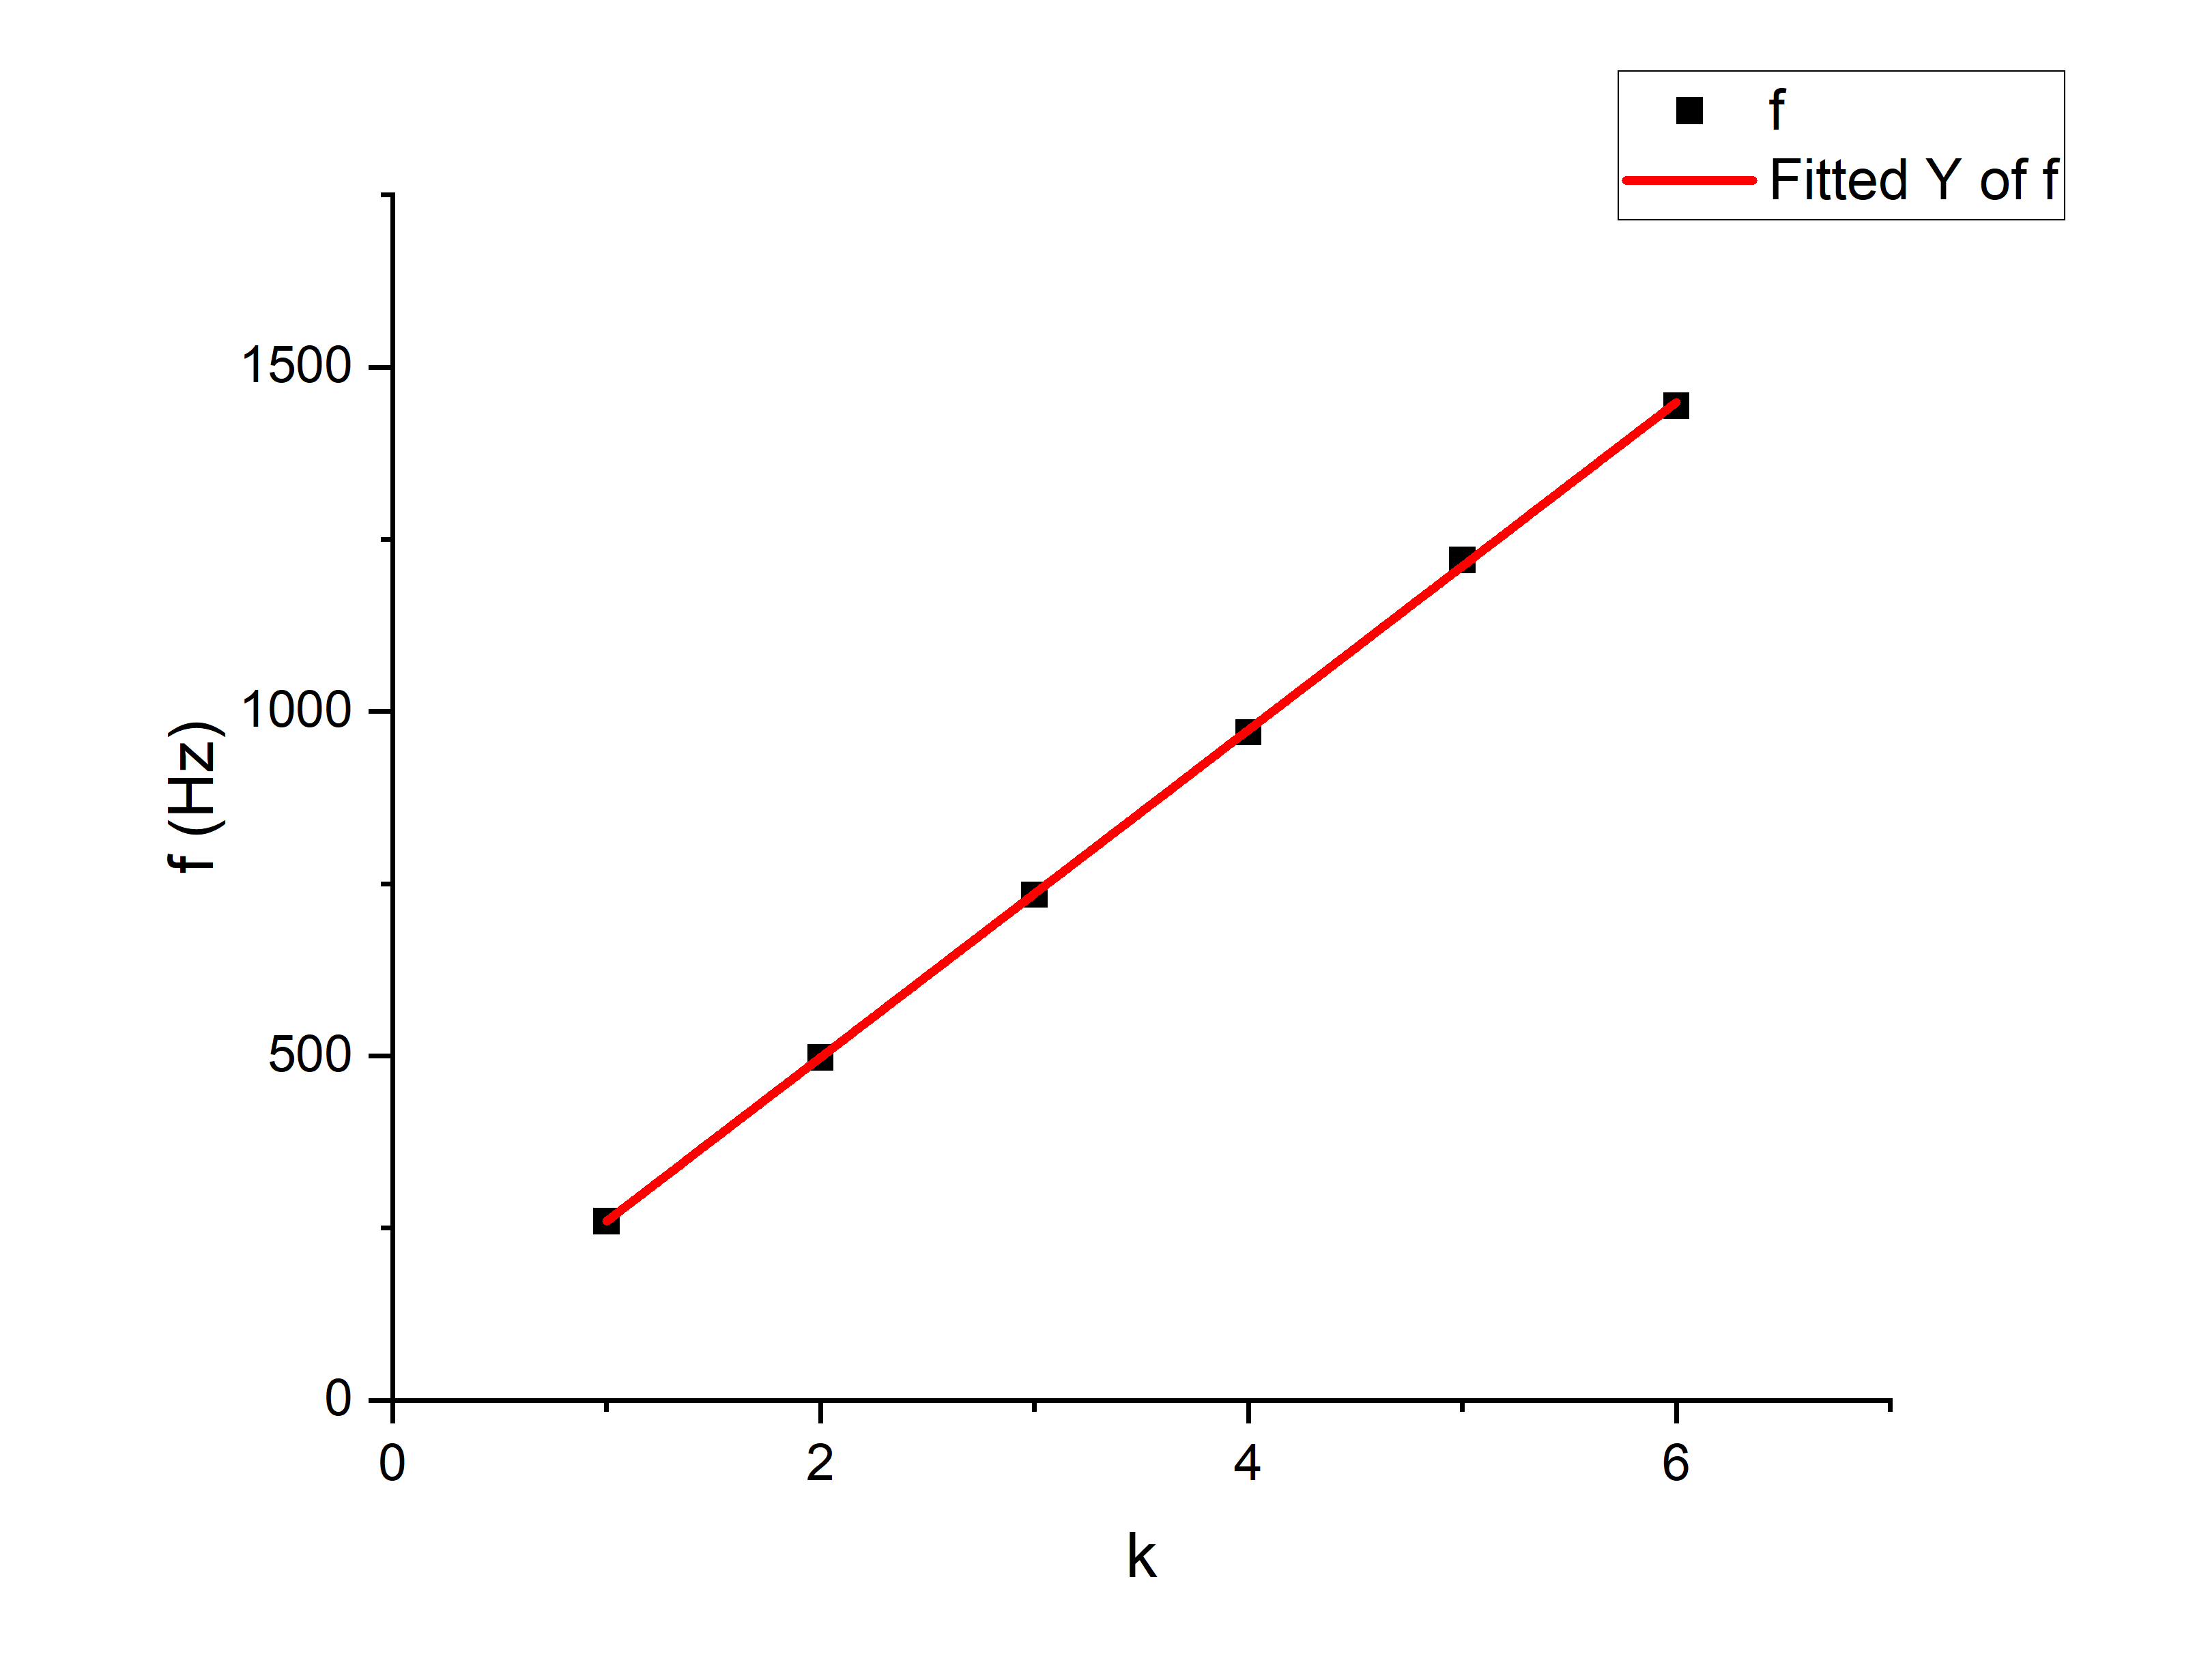
\includegraphics[width = 0.5\textwidth]{labphoto22.png}
\caption{График зависимости разности частот от номера резонанса при $T_6$}
\end{center}
\end{figure}

\begin{figure}
\begin{center}
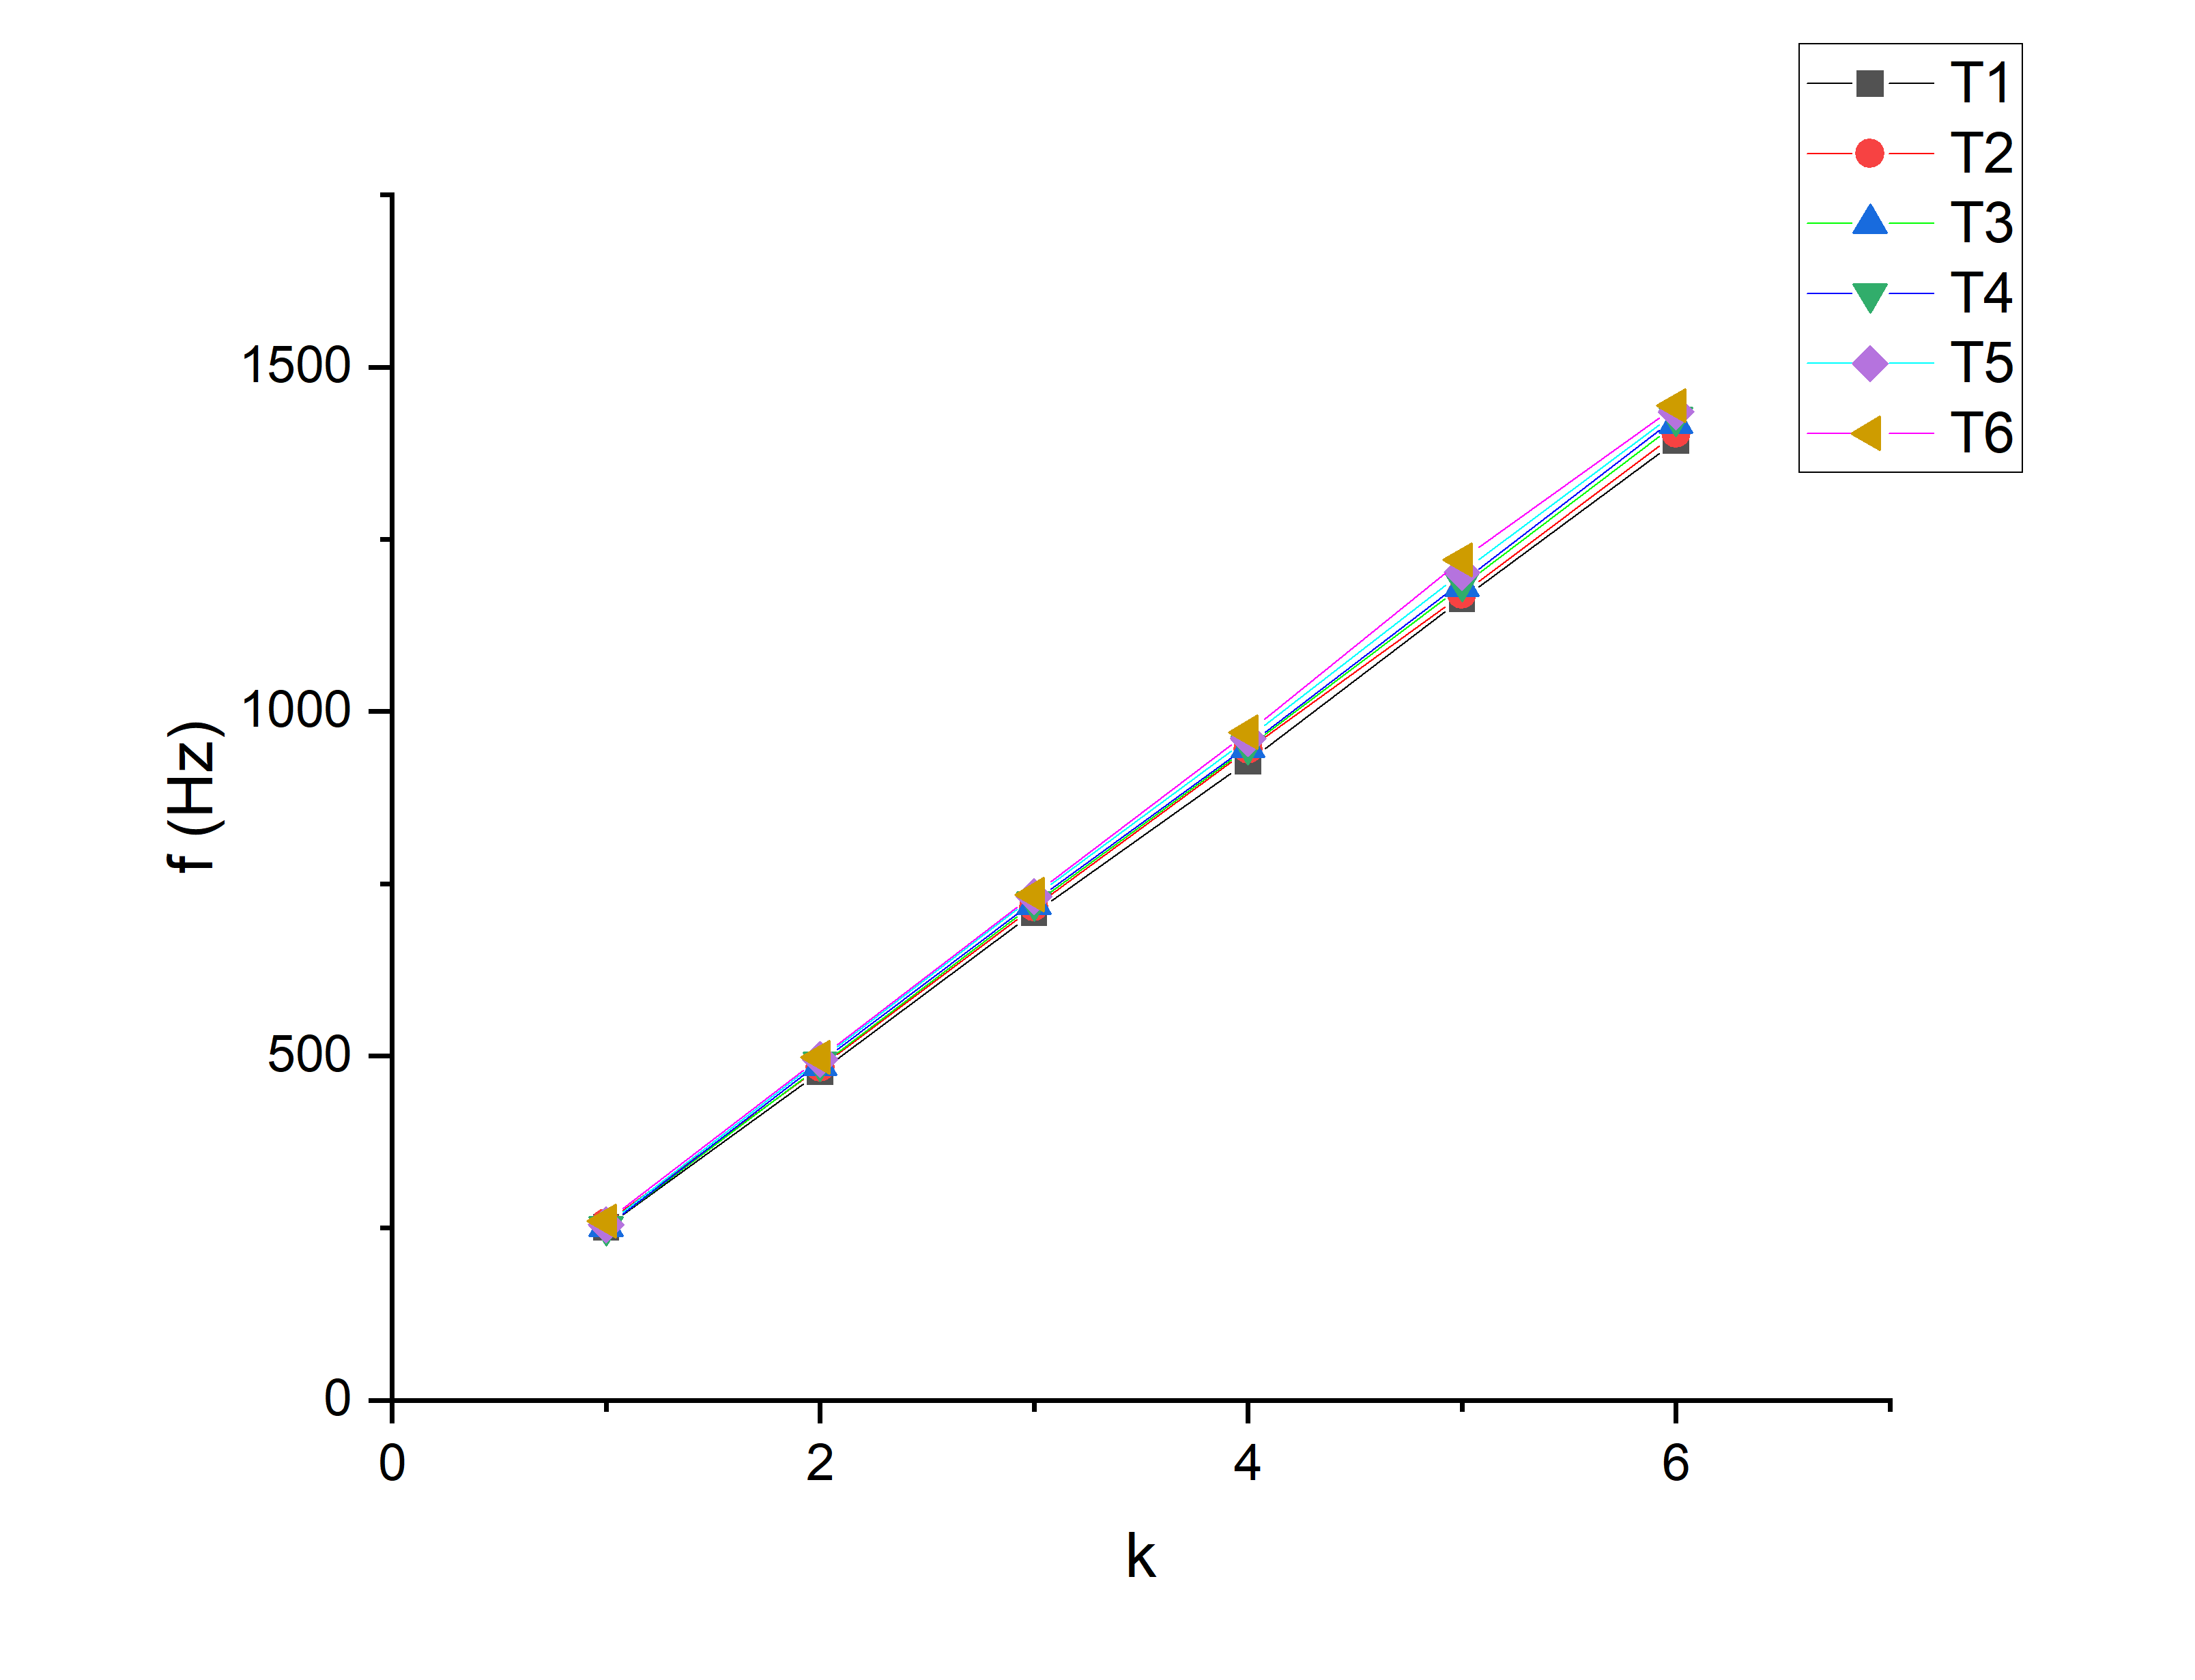
\includegraphics[width = 0.5\textwidth]{labphoto23.png}
\caption{График зависимости разности частот от номера резонанса при всех температурах вместе}
\end{center}
\end{figure}
\newpage
Угловые коэффициенты прямых соответственно равны:
\[
	a_1 = 228.22\ c^{-1} \quad a_2 = 229.2\ c^{-1}, \quad a_3 = 232.74\ c^{-1}, \quad a_4 = 234.08\ c^{-1}, 
\]
\[	
	\quad a_5 = 235.74\ c^{-1}, \quad a_6 = 237.77\ c^{-1}.
\]
Рассчитаем скорость звука и показатель адиабаты при каждой температуре по формулам (1) и (5):
\\
\begin{center}
\begin{tabular}{|c|c|c|}
\hline $T,\ K$ & $c,\ \text{м/с}$ & $\gamma$ \\\hline
$296$ & $346.03$ & $1.411$ \\\hline
$301$ & $349.08$ & $1.413$ \\\hline
$306.1$ & $352.19$ & $1.415$ \\\hline
$311.2$ & $354.92$ & $1.417$ \\\hline
$316.1$ & $358.29$ & $1.417$ \\\hline
$321$ & $361.28$ & $1.418$ \\\hline
\end{tabular}
\end{center}

Оценим погрешности:
\[
\varepsilon_{T} = 0.005 = 0.3\%
\]
\[
\varepsilon_{f} = 0.008 = 0.9\%
\]
\[
 \varepsilon_c = \sqrt{\varepsilon_{T}^2 + \varepsilon_{f}^2} = 0.0104 = 1.04\%
\]
\[
	\varepsilon_{\gamma} = 2 \varepsilon_c + \varepsilon_T = 0.0311 = 3.11\%
\]
Конечный ответ:
\[
	\boxed {\gamma = 1.415 \pm 0.05}
\]
Табличное значение:
\[
	\boxed {\gamma_{\text{табл}} = 1.403}
\]

\section{Вывод}
В этом эксперименте мы нашли удельную теплоемкость воздуха. Мы использовали звуковую волну в воздухе и изменили температуру, чтобы получить другое значение скорости звука. Получив константу при 6 различных температурах, мы взяли среднее значение и увидели, что оно очень близко к нашему табличному значению. Наша последняя экспериментальная ошибка почти \textbf{1.2} процент.


\end{document}